\documentclass[a4paper]{article}

\usepackage[english]{babel}
\usepackage{microtype}
\usepackage{graphicx}
\usepackage{amsmath}
\usepackage{index}

\makeindex
\graphicspath{/home/maxence/TP_CN/TP3_mini_robo/figures/commande position/jpeg}

\begin{document}
	\title{\large{\textbf{Compte rendu TP3}}}
	\title{\textbf{Robot Khepera}}
	\author{Arthur VAIN, Valentin Dosias, Maxence NEUS}
	\date{}
	
	\maketitle
	\newpage
	
	\tableofcontents
	\newpage
	
	\section{Introduction}
	L'objectif de ce TP est l'étude des différentes actions d'un régulateur PID à travers 2 commandes différentes: la commande en position et la commande en vitesse.
	
	Le robot étudié sera un robot mobile de type Khepera II possédant 2 roues motrices pilotés par des moteurs à courant continu grâce auxquels nous commanderons celui-ci.
	Pour ce faire, nous communiquerons avec ce robot à via une liaison série en utilisant Matlab 
	
	\section{Etude préliminaire}
	
	\section{Etude experimentale}
	\subsection{PID pour la commande en position}
	
	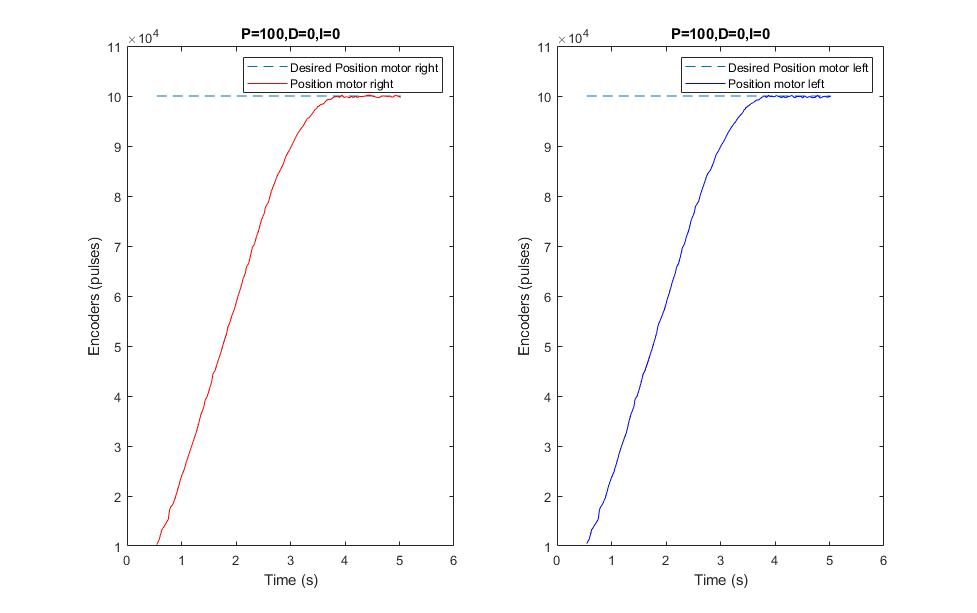
\includegraphics[width=5cm]{100_0_0.jpg}
	
	\subsection{PID pour la commande en vitesse}
	\subsection{Conclusion}
	P: Proportionnel, ce paramètre va gérer un gain brut. En général, plus il sera grand, plus il atteindra rapidement
	la valeur de la commande (voir trop rapidement et risque le plantage du robot ainsi que des dépassement de la commande)
	Il vas faire un gain constant à toutes les réactions du robot, il va surtout influer sur la rapidité.
		
	I: intégral, il va surtout influer sur la précision (de la commande vitesse ainsi que la commande position), il influe très peu sur la rapidité du système et un peu sur la stabilité. En effet, ce paramètre influe beaucoup sur la précision du système et nous permet de supprimer l'erreur constante si celle-ci est présente. Cette erreur constante est visible en zoomant sur les courbes, on remarque alors une erreur constante qu'il faut corriger.
	
	D: différentiel, il agit très peu sur la rapidité, un peu sur la précision mais influe énormément sur la stabilité. En effet, lors d'une perturbation, un changement brutal sera appliqué au système, donc une dérivée importante. C'est sur ce paramètre que l'on corrige le mieux ces perturbations.
	Attention, si il est trop fort, celui-ci risque juste de rendre le système instable.
	

\end{document}